% 2008 年陕西卷文科第 10 题：α⊥β，α∩β=l，A∈α、B∈β，A、B 到 l 的距离为 a、b，
%   AB 与 α、β 所成角为 θ、φ，射影长 m、n。
% 来源 PDF：gaokaomath-src/普通高考/2008/2008陕西文.pdf
% SHA-256：a0e35ce2cc6835012265595cf3b3fefa10f81e868623d594f4dddc786905c6ad
% 原页：2008陕西文.pdf 第 1 页（A3 三栏）第 2 栏，书页码 477。
% 重绘依据：按原页画两个互相垂直的半平面，交线 l 竖置；A 在竖平面 α 内、距 l 为 a，
%   B 在水平面 β 内、距 l 为 b，AB 连线，A 到 l 的垂足与 B 到 l 的垂足均画出。
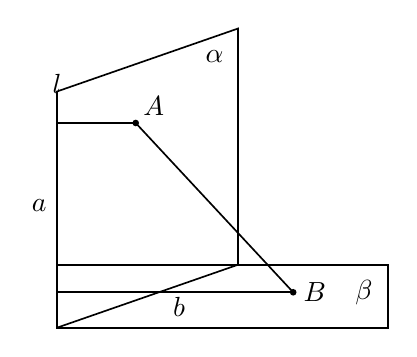
\begin{tikzpicture}[scale=1.0, semithick, every node/.style={inner sep=1.5pt}]
  % α（竖直半平面）
  \draw (0,0) -- (0,3.0) -- (2.3,3.8) -- (2.3,0.8) -- cycle;
  \node at (2.0,3.45) {$\alpha$};
  % β（水平半平面）
  \draw (0,0) -- (0,0.8) -- (4.2,0.8) -- (4.2,0) -- cycle;
  \node at (3.9,0.45) {$\beta$};
  % 交线 l
  \draw[line width=1.0pt] (0,0) -- (0,2.9) node[above] {$l$};

  \coordinate (A) at (1.0,2.6);
  \coordinate (Ap) at (0,2.6);
  \coordinate (B) at (3.0,0.45);
  \coordinate (Bp) at (0,0.45);

  \draw (A) -- (Ap);
  \draw (B) -- (Bp);
  \draw (A) -- (B);

  \fill (A) circle (1.2pt); \node[above right=1pt] at (A) {$A$};
  \fill (B) circle (1.2pt); \node[right=2pt] at (B) {$B$};
  \node[below left=1pt] at (Ap) {};
  \node[left=2pt] at (0.0,1.55) {$a$};
  \node[below] at (1.55,0.45) {$b$};
\end{tikzpicture}
